% !TEX TS-program = pdflatex
% !TEX encoding = UTF-8 Unicode

% This is a simple template for a LaTeX document using the "article" class.
% See "book", "report", "letter" for other types of document.

\documentclass[11pt]{article} % use larger type; default would be 10pt

\usepackage[utf8]{inputenc} % set input encoding (not needed with XeLaTeX)

%%% Examples of Article customizations
% These packages are optional, depending whether you want the features they provide.
% See the LaTeX Companion or other references for full information.

%%% PAGE DIMENSIONS
\usepackage{geometry} % to change the page dimensions
\geometry{letterpaper} % or letterpaper (US) or a5paper or....
\geometry{margin=1in} % for example, change the margins to 2 inches all round
% \geometry{landscape} % set up the page for landscape
%   read geometry.pdf for detailed page layout information

\usepackage{graphicx} % support the \includegraphics command and options
\usepackage{hyperref}

\usepackage[parfill]{parskip} % Activate to begin paragraphs with an empty line rather than an indent

%%% PACKAGES
%\usepackage{booktabs} % for much better looking tables
\usepackage{array} % for better arrays (eg matrices) in maths
%\usepackage{paralist} % very flexible & customisable lists (eg. enumerate/itemize, etc.)
\usepackage{verbatim} % adds environment for commenting out blocks of text & for better verbatim
%\usepackage{subfig} % make it possible to include more than one captioned figure/table in a single float
% These packages are all incorporated in the memoir class to one degree or another...

%%% HEADERS & FOOTERS
\usepackage{fancyhdr} % This should be set AFTER setting up the page geometry
\pagestyle{fancy} % options: empty , plain , fancy
\renewcommand{\headrulewidth}{0pt} % customise the layout...
\lhead{}\chead{}\rhead{}
\lfoot{}\cfoot{\thepage}\rfoot{}

%%% END Article customizations


%%% The "real" document content comes below...

\title{Experimental analysis of heat transfer properties of an enclosure}
\author{}
\date{} % Activate to display a given date or no date (if empty),
         % otherwise the current date is printed 

\begin{document}
\maketitle

%\begin{quote}
%Wise quote here.\\ \hbox{}\hfil -- {\em A Wise One}
%\end{quote}

\section{Introduction}

In this lab, you will develop a thermal model of an enclosure, which is an important early step in designing a climate control system. Indeed, one of the most important tasks of an engineer is to create system models that faithfully represent the physics with as little complication as necessary. Such models can then be used to test control algorithms, estimate performance, and determine important control parameters. Though we’re focusing on building a greenhouse, the theory here has many applications: a home heating system, climate control in a car, or heat removal in a server room packed with computers.

You’ll start by performing experiments on a small enclosure -- in this case a small plastic container (about as low-tech as we can get). As part of the lab, you will use an oscilloscope and apply basic electrical theory to collect experimental data from a temperature sensor. You will then use the data to parameterize a thermodynamic model. In the next few of weeks, you’ll apply these techniques to the design of your greenhouse.

Though we’re focusing on a physical prototype, thermal systems are usually characterized using theoretical models. When designing a large building (or even a greenhouse), it would not make sense to build the structure, test a bunch of heating systems, and then pick one to install. Because the procedure is so common, there are entire building simulation programs dedicated to modelling heating and cooling. Indeed, you’re asked to make an estimate of the thermal characteristics of your system from published sources in the pre-lab. But since this is a class in electromechanical systems, we’ll use the physical prototype to motivate the introduction to some common electronic concepts.

\subsection*{Objectives}

Upon successful completion of this module, the student should be able to:
\begin{itemize}
\item Apply basic principles of electricity to calculate current and power,
\item Demonstrate understanding of the principles of a voltage divider,
\item Demonstrate the use of a thermistor for measuring temperature,
\item Use an oscilloscope to read voltages,
\item Use an Arduino to gather time-series voltage data, and
\item Use energy principles to develop and parameterize a first-order thermodynamic model.%, and
%\item Design and test a heating system for an enclosure, given a set of constraints, and
%\item Estimate uncertainties in a thermodynamic model.
\end{itemize}

\section{Preparation}
%\subsection*{Background materials}

There are a number of topics to cover before coming to lab. In addition to the background material in this handout, be sure to review the following before coming to lab:

\begin{description}
\item [Basic laws of circuits and resistive elements.] There’s a decent overview in this \href{https://learn.sparkfun.com/tutorials/resistors}{\underline{SparkFun tutorial}}.
\item [Thermistors.] Read Sections 13 - 13.3 in the reading posted on collab.
\item [Use of the Digilent Analog Discovery.] Watch the \href{https://www.youtube.com/playlist?list=PLSTiCUiN_BoJ0ZwU5wj73OO_7BI2NcihM}{\underline{introductory videos}} and \emph{install the Waveforms software}. You will not be using the Arbitrary Waveform Generator in this lab, so you may skip Video 4 for now. {\bf I cannot understate the usefulness of the oscilloscope!}
\item If you’ve never used a multimeter before, this \href{https://learn.sparkfun.com/tutorials/how-to-use-a-multimeter/}{\underline{SparkFun tutorial}} is very comprehensive. Concentrate on the parts that explain how to do measurements.
\end{description}
{\bf You must complete the pre-lab worksheet in Section~\ref{sec:prelab} and turn it in at the beginning of lab.} The pre-lab is an individual assignment.

\subsection{Thermodynamic model}

Your goal is to develop a model of your greenhouse that can be used to design an appropriate heating system. Specifically, you will want to size the heating element(s) so that a minimum temperature can be maintained for all expected weather conditions. Here, you will start with a simplified, first-order model of the heat transfer process. It is called first-order because the resulting ordinary differential equation, the \emph{governing equation},\footnote{The governing equation is the most basic equation, usually a differential equation, that describes the physics of a system.} will have only first derivatives in it. First-order o.d.e.'s are the simplest form of o.d.e. and are easy to solve, even if you haven't completed a course in differential equations.

Imagine an enclosure at some internal temperature, $T_{i}$, that is placed in an environment at another temperature, which we'll call $T_{o}$. In general, energy in the form of heat will flow either into or out of the enclosure, depending on the relative temperatures. The rate at which energy is transferred is dependent on many factors, including the temperature difference, the insulation around the enclosure, and the leakiness of the enclosure. In addition, the enclosure may have some internal addition of energy, for example from a heater.

If we draw a \emph{control volume} around the enclosure as shown in Figure~\ref{fig:control.volume}, then we can perform an \emph{energy balance} in that control volume. As you remember from your physics classes (you do remember them, yes?), conservation of energy requires that the change in energy, $E$, in the control volume is equal to the rate at which energy flows across the boundary as heat, $Q_{s}$, plus the rate at which heat is added internally, $Q_{i}$.\footnote{To be clear, $Q$ is formally a rate of energy flow, or heat, which has units of Watts.} Mathematically, this is expressed as:
\[
\frac{dE}{dt} = Q_{s} + Q_{i}
\] 
%
Note that we count heat \emph{entering} the system as a positive quantity; when heat is leaving the system, energy flows are negative.

\begin{figure}
\centering
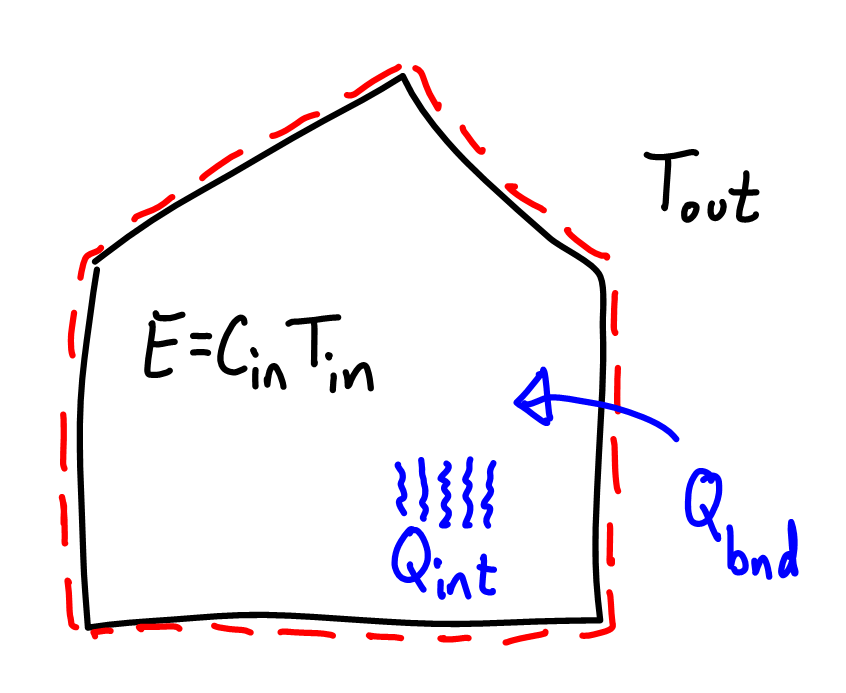
\includegraphics[width=2.5in ]{figures/control_volume.png}
%\end{center}
\caption{Control volume (shown in dashed red) for our thermodynamic analysis.}
\label{fig:control.volume}
\end{figure}

The heat capacity relates the temperature of a mass to the amount of thermal energy it contains. In reality, it is a complex quantity related to the masses of the individual components (e.g., air, metal, glass, plastic) and their thermodynamic properties. For our purposes, we'll just lump everything together and stipulate:
\[
E = C_{i}T_{i}
\]
%
where $C_{i}$ is the lumped heat capacitance. 

To calculate the heat moving across the boundary, $Q_{s}$, one can sum up the contribution of each type of boundary material by multiplying its thermal conductance, typically denoted by $U$ in structural applications, by the area of that material and the temperature difference. That is,
\[
Q_{s} = \sum_jU_jA_j\left(T_{o} - T_{i}\right)
\] 
%
Again, note that positive heat flow is into the system: if it's warmer outside than in, then $Q_{s}>0$. The greater the differential, the greater the rate at which energy flows. We'll simplify things further by defining an overall heat transfer coefficient for a given structure, $K_s$, as:
\[
K_s\equiv  \sum_jU_jA_j
\]
%
thus, $Q_{s}$ can be simplified to,
\[
Q_{s} = K_s\left(T_{o} - T_{i}\right)
\]
We can substitute the expressions above into our energy balance equation to get:
\[
\frac{dE}{dt} = C_{i}\frac{dT_{i}}{dt} = K_s\left(T_{o} - T_{i}\right) + Q_{i}
\]
which can be rearranged slightly to produce:
\begin{equation}
C_{i}\frac{dT_{i}}{dt} + K_s T_{i}=  K_sT_{o} + Q_{i}
\label{eq:gov.eq}
\end{equation}

If you've had a class in differential equations, you should recognize this as a first-order, linear, non-homogeneous, ordinary differential equation with constant coefficients. If you haven't, some of those terms might not mean much to you, but just note that under certain conditions, the equation is easily solved. Specifically, if we stipulate that both the outside temperature and internal heat are constant, we can readily solve the equation to get:

\begin{equation}
T_i(t) = T_i(0)e^{-\frac {K_s} {C_i} t}  +  \left[T_o+\frac {Q_i} {K_s}\right]\left[1-e^{-\frac {K_s} {C_i} t} \right]
\label{eq:solution}
\end{equation}
%
Physically, we can interpret the solution as follows: the first term on the right hand side (r.h.s) is the effect of the initial temperature, $T_{i}(0)$, whose influence diminishes as time goes on (as seen from the exponential). When $t=0$, all of the exponential terms are $1$, and so the only non-zero term on the r.h.s. is the initial temperature. As time goes on, the effect of the initial temperature approaches zero. The second term on the r.h.s. captures the effects of ``forcing'', whether from a temperature differential between the inside and outside or from internal heating. As time goes to infinity, the exponential terms will go to zero, and the only remaining terms will be constants related to $T_{o}$ and $Q_{i}$ (remember, we assumed that $T_{o}$ and $Q_{i}$ are constant). Because the temperature will not change any further under those conditions, the resulting temperature is called the \emph{steady-state} solution.

Before continuing, substitute Equation~\ref{eq:solution} into the governing equation to verify that the above equation is indeed a solution to the governing equation. Determine the steady-state solution by taking the limit of Eq.~\ref{eq:solution} as $t\rightarrow \infty$. Separately, note that if the temperature isn’t changing, the derivative $dT/dt\equiv 0$ in Equation~\ref{eq:gov.eq}; if you set the derivative in the governing equation to 0, you should be able to generate the same steady-state solution. The pre-lab exercises ask you to do just that.

There are two unknown physical parameters that you need to determine for your model: $C_{i}$ and $K_s$. They both show up in the exponential (time) term, but only $K_s$ appears in the steady-state solution. Thus, you can determine $K_s$ by adding energy with a heater and observing the interior temperature over a long period. Once $K_s$ is known, you can use the transient response over short periods of time to determine $C_{i}$. 

\subsection{The Voltage Divider}

To read the temperature of your system, you’ll make use of a thermistor -- a device that changes resistance based on temperature -- in something called a \emph{voltage divider}, which will translate changes in resistance to changes in voltage, which are easily read by microcontrollers. The voltage divider is easily the most common circuit that you will encounter in electronics. Luckily, it is also a fairly simple circuit, and you should get to the point where analyzing one is practically automatic. Consider the circuit in Figure~\ref{fig:voltage.divider}, where a voltage potential is applied to two resistors connected in series. We wish to find the voltage in between them, at point B. If no current flows in or out at point B -- a practical occurrence in many situations -- the current through each resistor must be equal to the current through the entire circuit,
\[
I_{A\rightarrow B} = I_{B\rightarrow C} = I_{A\rightarrow C}
\]
which from Ohm’s Law gives,
\[
\frac {V_A - V_B} {R_1} = \frac {V_B - V_C} {R_2} = \frac {V_A - V_C} {R_1 + R_2}
\]
A little rearrangement of the second equality leads to
\[
\frac {V_B - V_C} {V_A- V_C} = \frac {R_2} {R_1 + R_2}
\]
or
\[
V_B= V_C+\left(V_A- V_C\right) \frac {R_2} {R_1 + R_2}
\]
which is just a line fit to the points as shown in Figure~\ref{fig:dividergraph}. Usually, \emph{but not always}\footnote{In particular, on quizzes...}, $V_C$ is ground, which if we take to be 0V yields,
\[
V_B =V_A  \frac {R_2} {R_1 + R_2}
\]
That is, the voltage at point B is just the input voltage, $V_A$, times the ratio of $R_2$ to the total resistance.
\begin{figure}
\centering
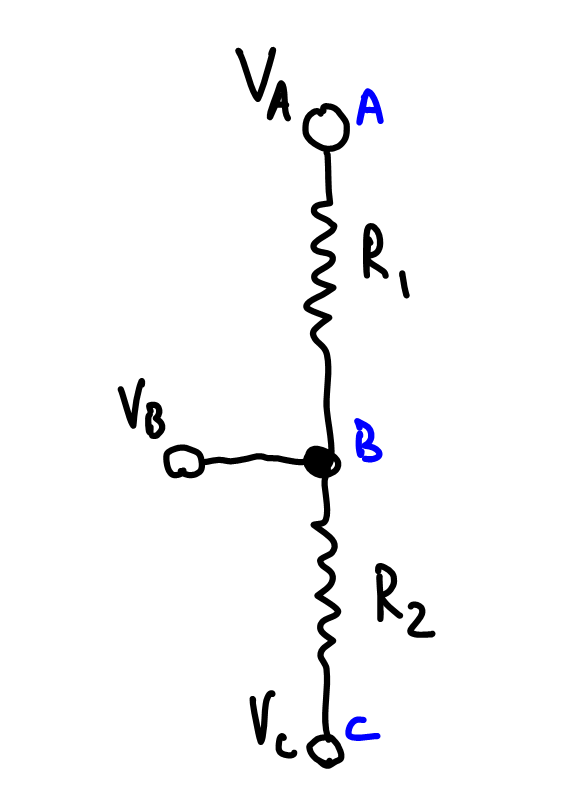
\includegraphics[width=2in]{figures/voltagedivider.png}
%\end{center}
\caption{A voltage divider. Please, control your excitement.}
\label{fig:voltage.divider}
\end{figure}

Care must be taken to ensure that no current leaves junction B through anything we might connect to it; otherwise, the voltage at point $B$ will change. For example, if $V_B$ is a reference voltage for another purpose, we’ll have to make sure that the current is negligible compared to that flowing through the resistors. The inputs on our oscilloscopes have extremely high resistances, so this is not a concern in this lab. In other cases, you can construct a buffer circuit to prevent changes in voltage.
\begin{figure}
\centering
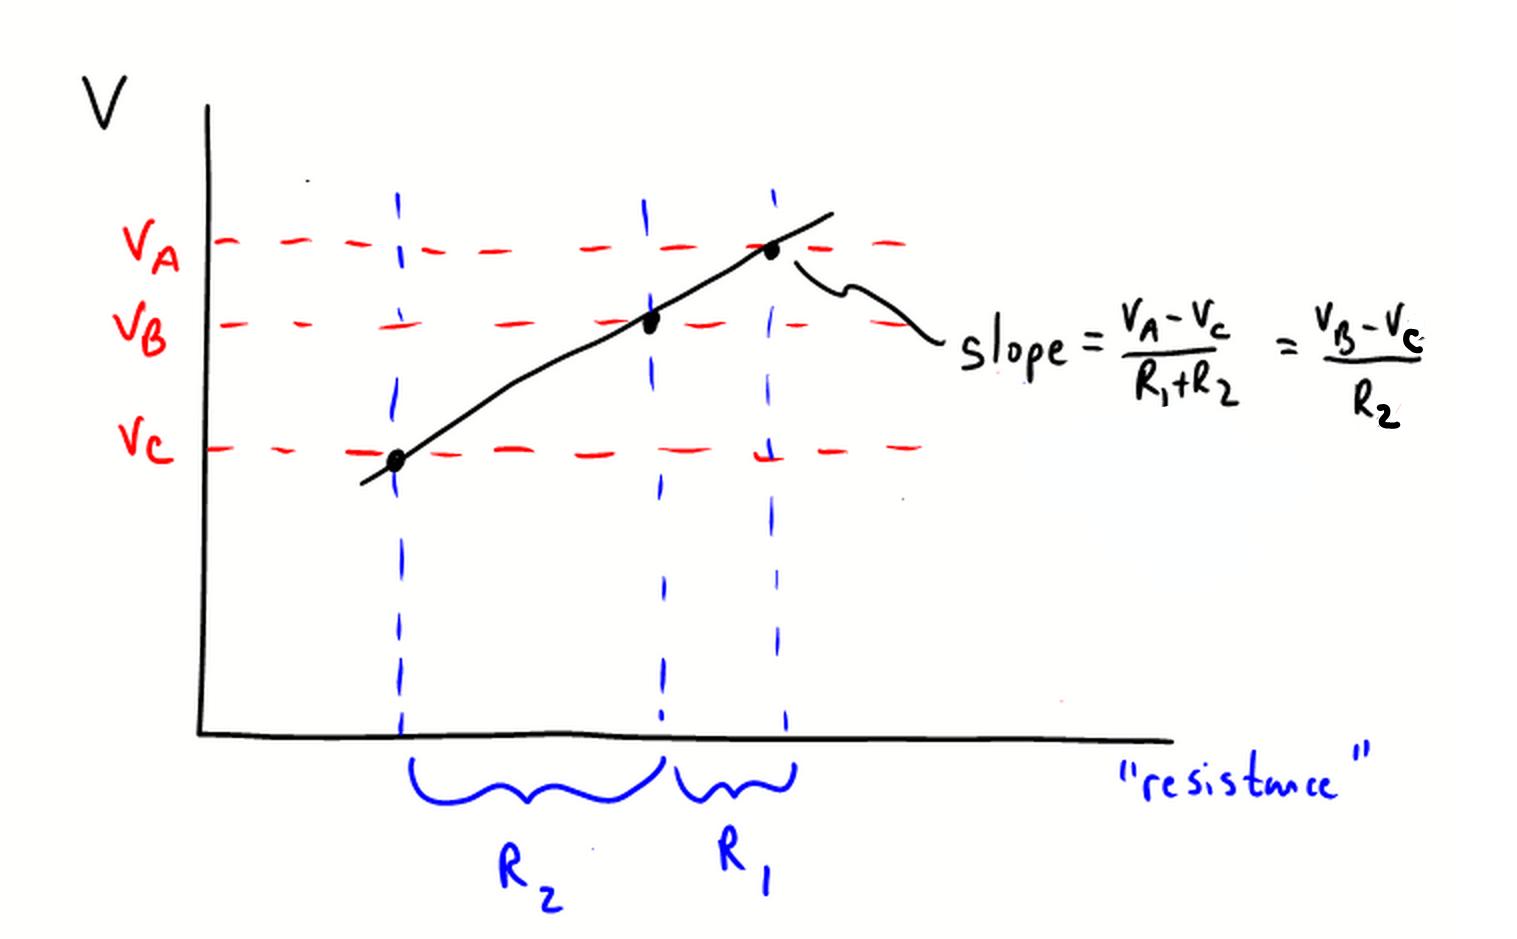
\includegraphics[width=4.5in]{figures/voltagegraph.png}
%\end{center}
\caption{A graphical interpretation of a voltage divider.}
\label{fig:dividergraph}
\end{figure}

\subsection{The thermistor}

The resistance of any resistor changes as a function of temperature. For many applications, the exact size of the resistor isn’t terribly important and so the temperature effects are safely ignored. When the exact resistance is important, the changes can be accounted for in the circuit design or compensated for afterwards in software. A \emph{thermistor}, on the other hand, is specifically designed to take advantage of the changes in resistance so that it can be used to \emph{measure} temperature. Thermistors are optimized to have predictable changes in resistance over a given range of temperatures. By putting the thermistor in one leg of a voltage divider, a change in temperature will ultimately result in a change in voltage, which is easily measured.

Over the limited range of temperatures we’ll see in this lab, the resistance of the thermistor can be approximated as,

\begin{equation}
R = R_0 e^{-B\left(\frac 1 {T_0} - \frac 1 T \right)}
\label{eq:thermistor}
\end{equation}
%
where $B$ is a constant specified by the manufacturer, and $R_0$ is the resistance measured at some specified temperature, $T_0$, in Kelvin. Manufacturers typically calibrate thermistors at 25C, but we’ll calibrate ours independently at room temperature, which will be slightly lower than that.

\subsection{The potentiometer}

A potentiometer is a common electrical component that allows the user to easily change the relative resistances between its contacts. A potentiometer (often simply called a “pot”) can either be used as a variable resistor (sometimes called a rheostat) or as a voltage divider. The resistance between the end terminals is fixed to some specified resistance ($10k\Omega$ is a popular size), while a third terminal, the \emph{wiper}, is allowed to slide along the resistive material between the ends; for a linear potentiometer, the resistance between the wiper and a given end is proportional to the distance between the contacts. By connecting one end terminal and the wiper to a circuit, one creates a variable resistor, which might be used, for example, for volume control of an amplifier. By applying a voltage differential across the end terminals, the wiper can be used as a variable voltage divider. Figure~\ref{fig:rheostat} shows a potentiometer configured as a variable resistor. Figure~\ref{fig:var.vd} shows a variable voltage divider.

\begin{figure}[htbp]
\begin{center}
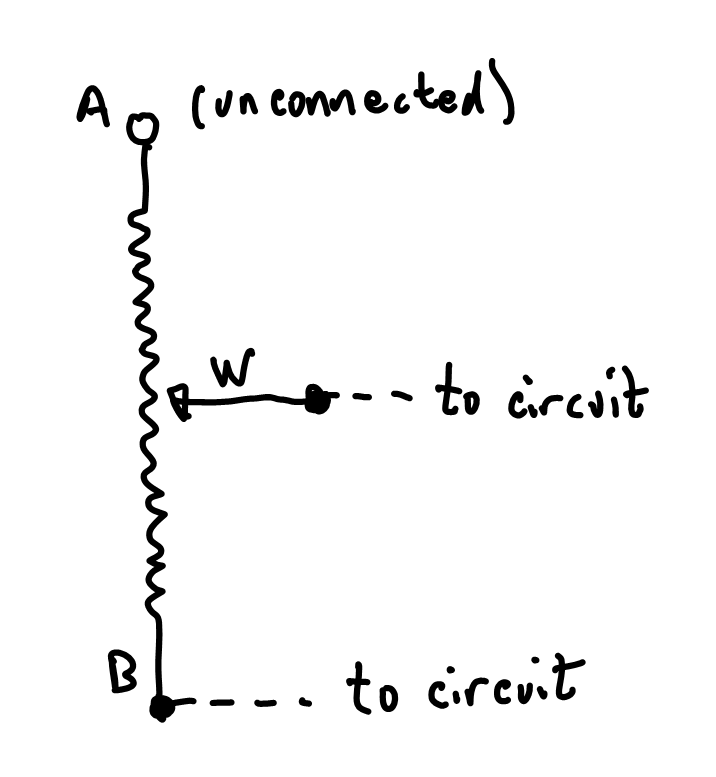
\includegraphics{figures/rheostat}
\caption{A variable resistor, or rheostat.}
\label{fig:rheostat}
\end{center}
\end{figure}

\begin{figure}[htbp]
\begin{center}
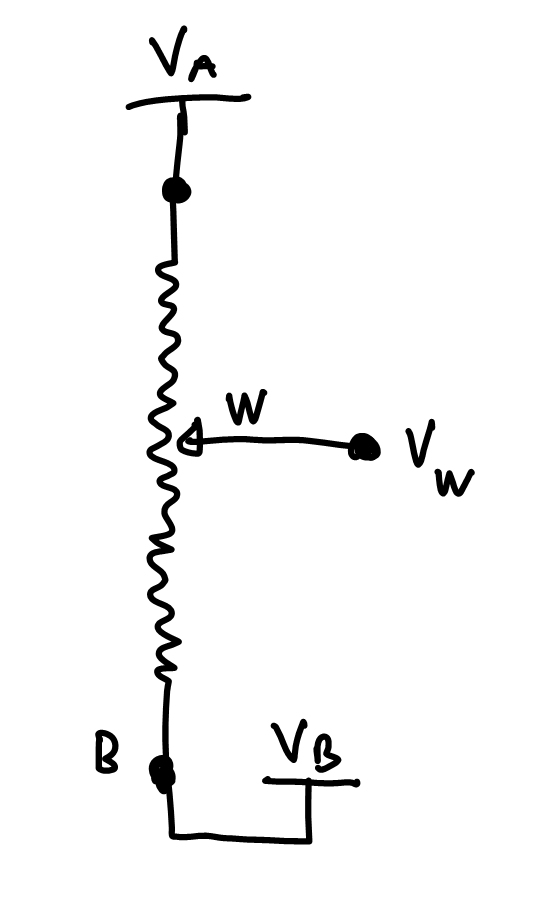
\includegraphics{figures/var_voltage_divider}
\caption{A variable voltage divider.}
\label{fig:var.vd}
\end{center}
\end{figure}

\section{In lab}

Your goal in this lab is to create a thermal model for an enclosure and determine the model parameters from experimental data. You’ll do this for a small enclosure and later apply the techniques to your actual greenhouse. You’ll measure the temperature using a thermistor configured as part of a voltage divider, which will allow you to calculate the resistance of the thermistor and thereby the temperature.

\section*{Using an oscilloscope and multimeter}

Before getting started on the temperature measurements, you’ll be introduced to two important tools for designing and testing circuits: the oscilloscope and the multimeter. The multimeter you’ll use in lab can measure many things, including voltage, resistance, and capacitance. Because it is digital, we will refer to it as a digital multimeter, or DMM. The Digilent Analog Discovery includes many tools: oscilloscope, arbitrary wave generator, power supply, voltmeter, and a bunch of digital tools. Here, we’ll use a potentiometer to demonstrate the concept of a voltage divider and you’ll become familiar with some of the functionality of the Analog Discovery.

\subsection*{Procedure}

\begin{enumerate}
\item Insert the leads from the $10k\Omega$ potentiometer on your workstation into the breadboard and connect the oscilloscope as shown in Figure~\ref{fig:potentiometer}.
%\item Connect the oscilloscope as shown. 
For this and many of the following labs, your life will be \emph{much} easier if you plug the oscilloscope leads into a central location and then use jumper wires to “probe” your circuit. It’s kind of a pain to keep the oscilloscope wires connected otherwise, and it’s much quicker to just move a jumper wire around.

\begin{figure}[htbp]
\begin{center}
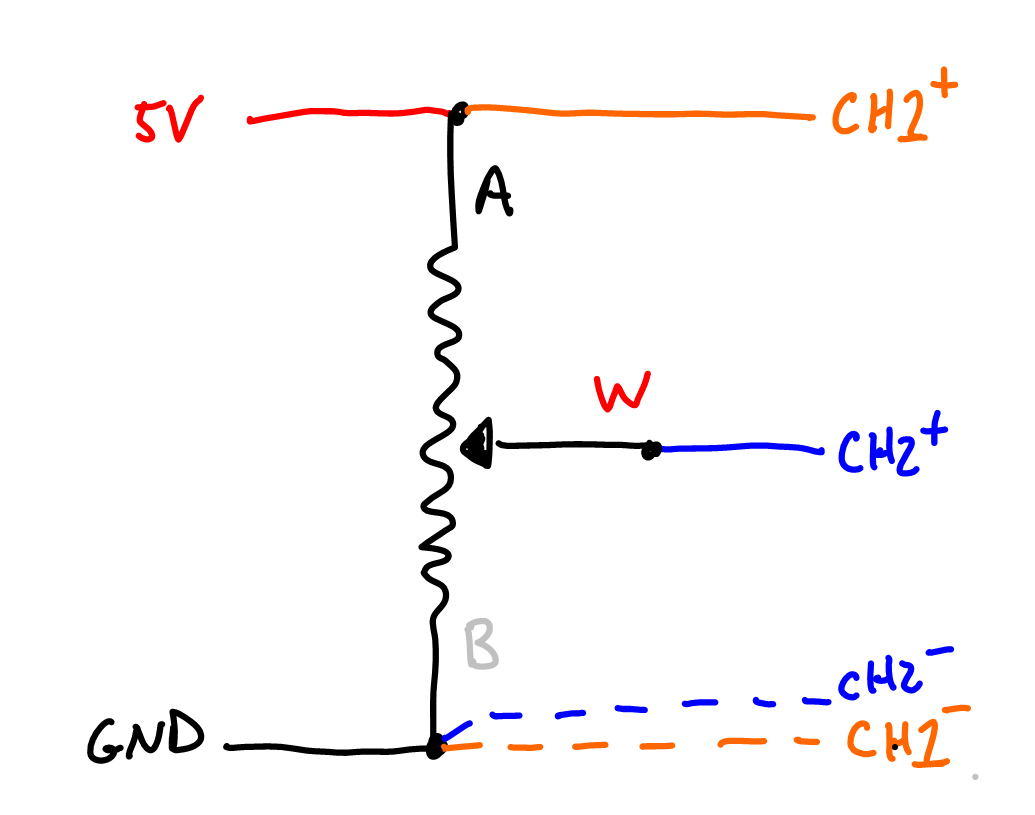
\includegraphics{figures/potentiometer}
\caption{Connections for the potentiometer, with the terminals labelled in the same convention as on your workstation.}
\label{fig:potentiometer}
\end{center}
\end{figure}

%\item Connect the 5V power supply from the oscilloscope to one side of the potentiometer. Connect the other to ground.
\item Open the oscilloscope software and start the oscilloscope. Since the 5V power line is not yet energized, you should see readings of 0V. Set the scale to 1V per division and the offset to -2V for both channels. Set the Trigger to “None”. 
\item From the main screen of the oscilloscope, turn on the +5V supply. You should see CH1 jump to somewhere around 5V. Note that the source is a nominal 5V, so it is important to measure the actual value.
\item Turn the potentiometer and observe CH2. What is happening?
\item Turn the potentiometer such that CH2 reads 3.5V. Pull the potentiometer leads out from the breadboard and, using the DMM, measure the resistance between each terminal and the wiper. {\bf It is imperative that whenever you measure resistance that the component in question be isolated from the circuit.} Otherwise, you certainly won’t get a meaningful reading and you might damage the multimeter.
\item Given the measured resistances, calculate the expected voltage at the wiper. How does it compare to the measured value?
\item Plug the potentiometer back into the breadboard and measure the voltage using the DMM. Note that for constant or slowly changing voltages, it is generally easier to use the DMM than an oscilloscope, but it is important that you know how to use both.
\end{enumerate}

\section*{Reading voltages with a microcontroller}

Here, you’ll use an Arduino Uno to read voltages instead of the oscilloscope. The oscilloscope is a critical tool for exploring and debugging, but using the Uno will make collecting the data significantly easier.\footnote{The oscilloscope can save data, but you can’t interact with it while it’s collecting data, so there’s too much risk something will go wrong and you’ll have to do the data collection all over.} We’ll talk much about how the Uno reads voltages in the future, but the short version is that the Uno has a built-in \emph{analog-to-digital converter}, or ADC. The ADC takes a voltage and turns it into a number using the formula:

\begin{equation}
result = floor \left( \frac{V}{V_{ref}} \times 1024\right)
\label{eq.adc}
\end{equation}
%
where $V$ is the voltage that you’re reading and $V_{ref}$ is the reference voltage that the microcontroller uses to compare to $V$. In this case $V_{ref}\approx 5V$. Why the formula has this form and how the ADC works is a subject for another day. Using the Uno, however, will allow you to easily collect data for later processing. Since we have yet to cover the details of the Uno, your instructor has provided a basic program for data collection.

\subsection*{Procedure}

\begin{itemize}
\item {\bf Disconnect the Analog Discovery from the circuit entirely} and build the circuit shown in Figure~\ref{fig:adc.uno}. Note that the Uno will be providing power to the circuit from the 5V pin.

\begin{figure}
\centering
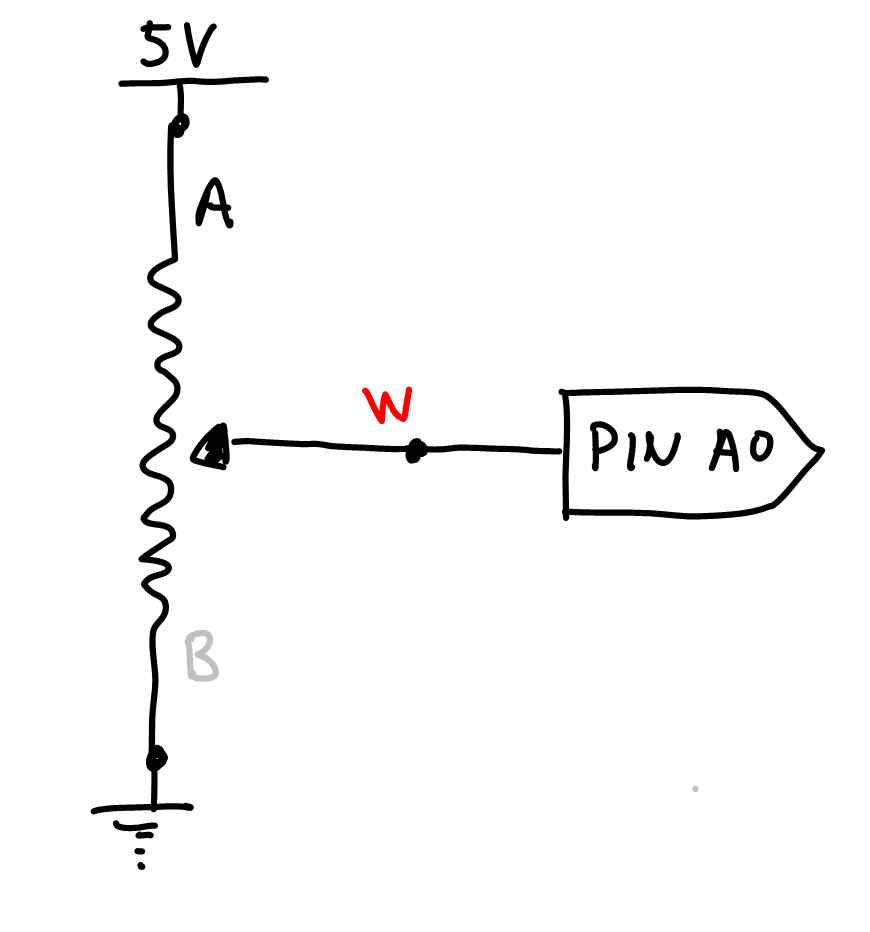
\includegraphics[width=3in ]{figures/adc}
\caption{Circuit for exploring the Uno’s ADC.}
\label{fig:adc.uno}
\end{figure}

\item Upload the program provided. When finished, open the Serial Monitor by clicking the icon in the upper right of the Arduino IDE. Two columns should start scrolling down the screen: the first is the time in seconds since the program has started, and the second the reading from the ADC (Equation~\ref{eq.adc}).
\item Using a DMM to measure voltage, adjust the potentiometer the wiper terminal measures 1.0V and note the ADC reading. Fill in the appropriate line in Table~\ref{tab:adc}.
\item Repeat the process for each of the values in Table~\ref{tab:adc}. How well do the actual and theoretical values compare?
\end{itemize}

\begin{table}[h]
\centering
\begin{tabular}{c|c|c}
\hline
%&\multicolumn{2}{c}{(Nominal 5V) AREF =    }\vline & \multicolumn{2}{c}{(External reference) AREF =    }\\
%\hline
Wiper voltage & Theoretical ADC reading & Actual ADC reading \\
\hline\hline
0V&&\\
\hline
1V&&\\
\hline
2V&&\\
\hline
3V&&\\
\hline
4V&&\\
\hline
5V&&\\
\hline
\end{tabular}
\caption{Record your ADC calculations here.}
\label{tab:adc}
\end{table}


\section*{Heat transfer experiment}

Here, you’ll apply the tools, techniques, and theory from above to build a thermodynamic model of a small enclosure.

To collect data for the model, you will be provided with the following supplies:
\begin{itemize}
\item A small plastic container (not your greenhouse -- that comes later),
\item A 10W, 6.2$\Omega$ power resistor,
\item A 12V “wall wart” power supply (2A max\footnote{It is a common misconception that the amperage rating on a power supply means it will put out that many amps. In actuality, the voltage supply will put out a (nominal) voltage and as much current as the load requires to maintain that voltage \emph{up to the rated current}. Exceeding the rated current may damage the power supply.}),
\item A $10k\Omega$ thermistor, model B57164K0103J, and
\item Basic electronic components to complete your circuits.
\end{itemize}

\subsection*{Procedure}
{\bf Read these directions thoroughly before you start the experiment.} Timing is important!
\begin{enumerate}
\item Measure the actual resistance of your power resistor and calculate the voltage needed to generate 8W of heat from it. Verify that you are not exceeding the 2A limit on your power supply.
\item If it hasn’t been done already, connect the 5.5mm/2.1mm output terminal of the power supply to the voltage regulator using the supplied adaptor. Use the standard convention of red for positive voltage and black for ground (negative). See Figure~\ref{fig:power.supply}.

\begin{figure}
\centering
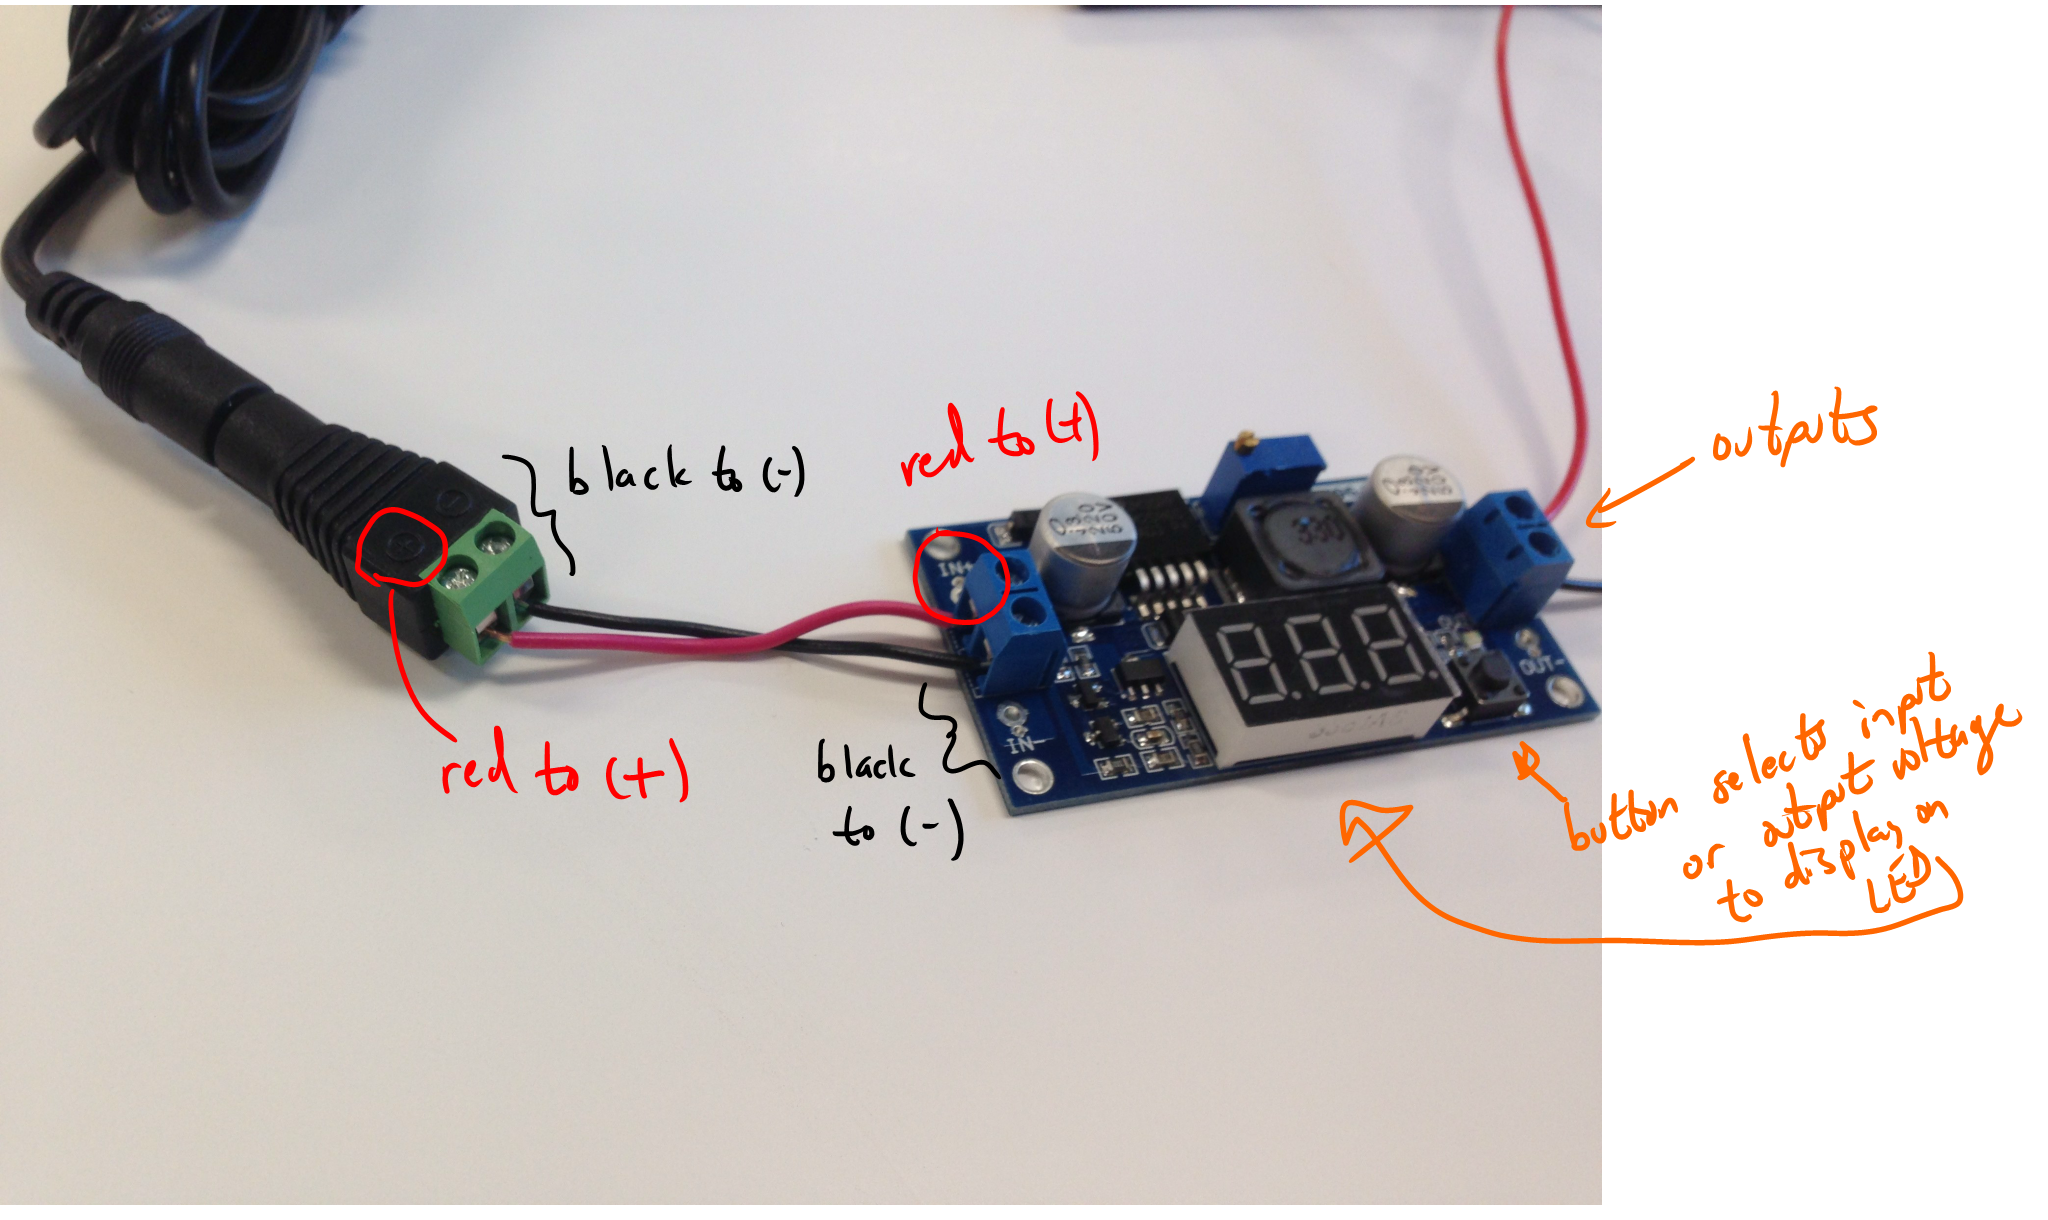
\includegraphics[width=4.5in ]{figures/powersupply}
\caption{Image showing power supply connections.}
\label{fig:power.supply}
\end{figure}

\item Plug in your power supply and the LED on the voltage regulator should light up. The LED can be toggled between input and output voltages. The input voltage should be around 12V (the rating on the supply). Adjust the output voltage to the value determined previously using the small screw on the face of the regulator.
\item Unplug the power supply and connect the power resistor to the output of the voltage regulator. Use a small breadboard, as shown in Figure~\ref{fig:power.resistor} to do this. Be careful not to short anything together!

\begin{figure}
\centering
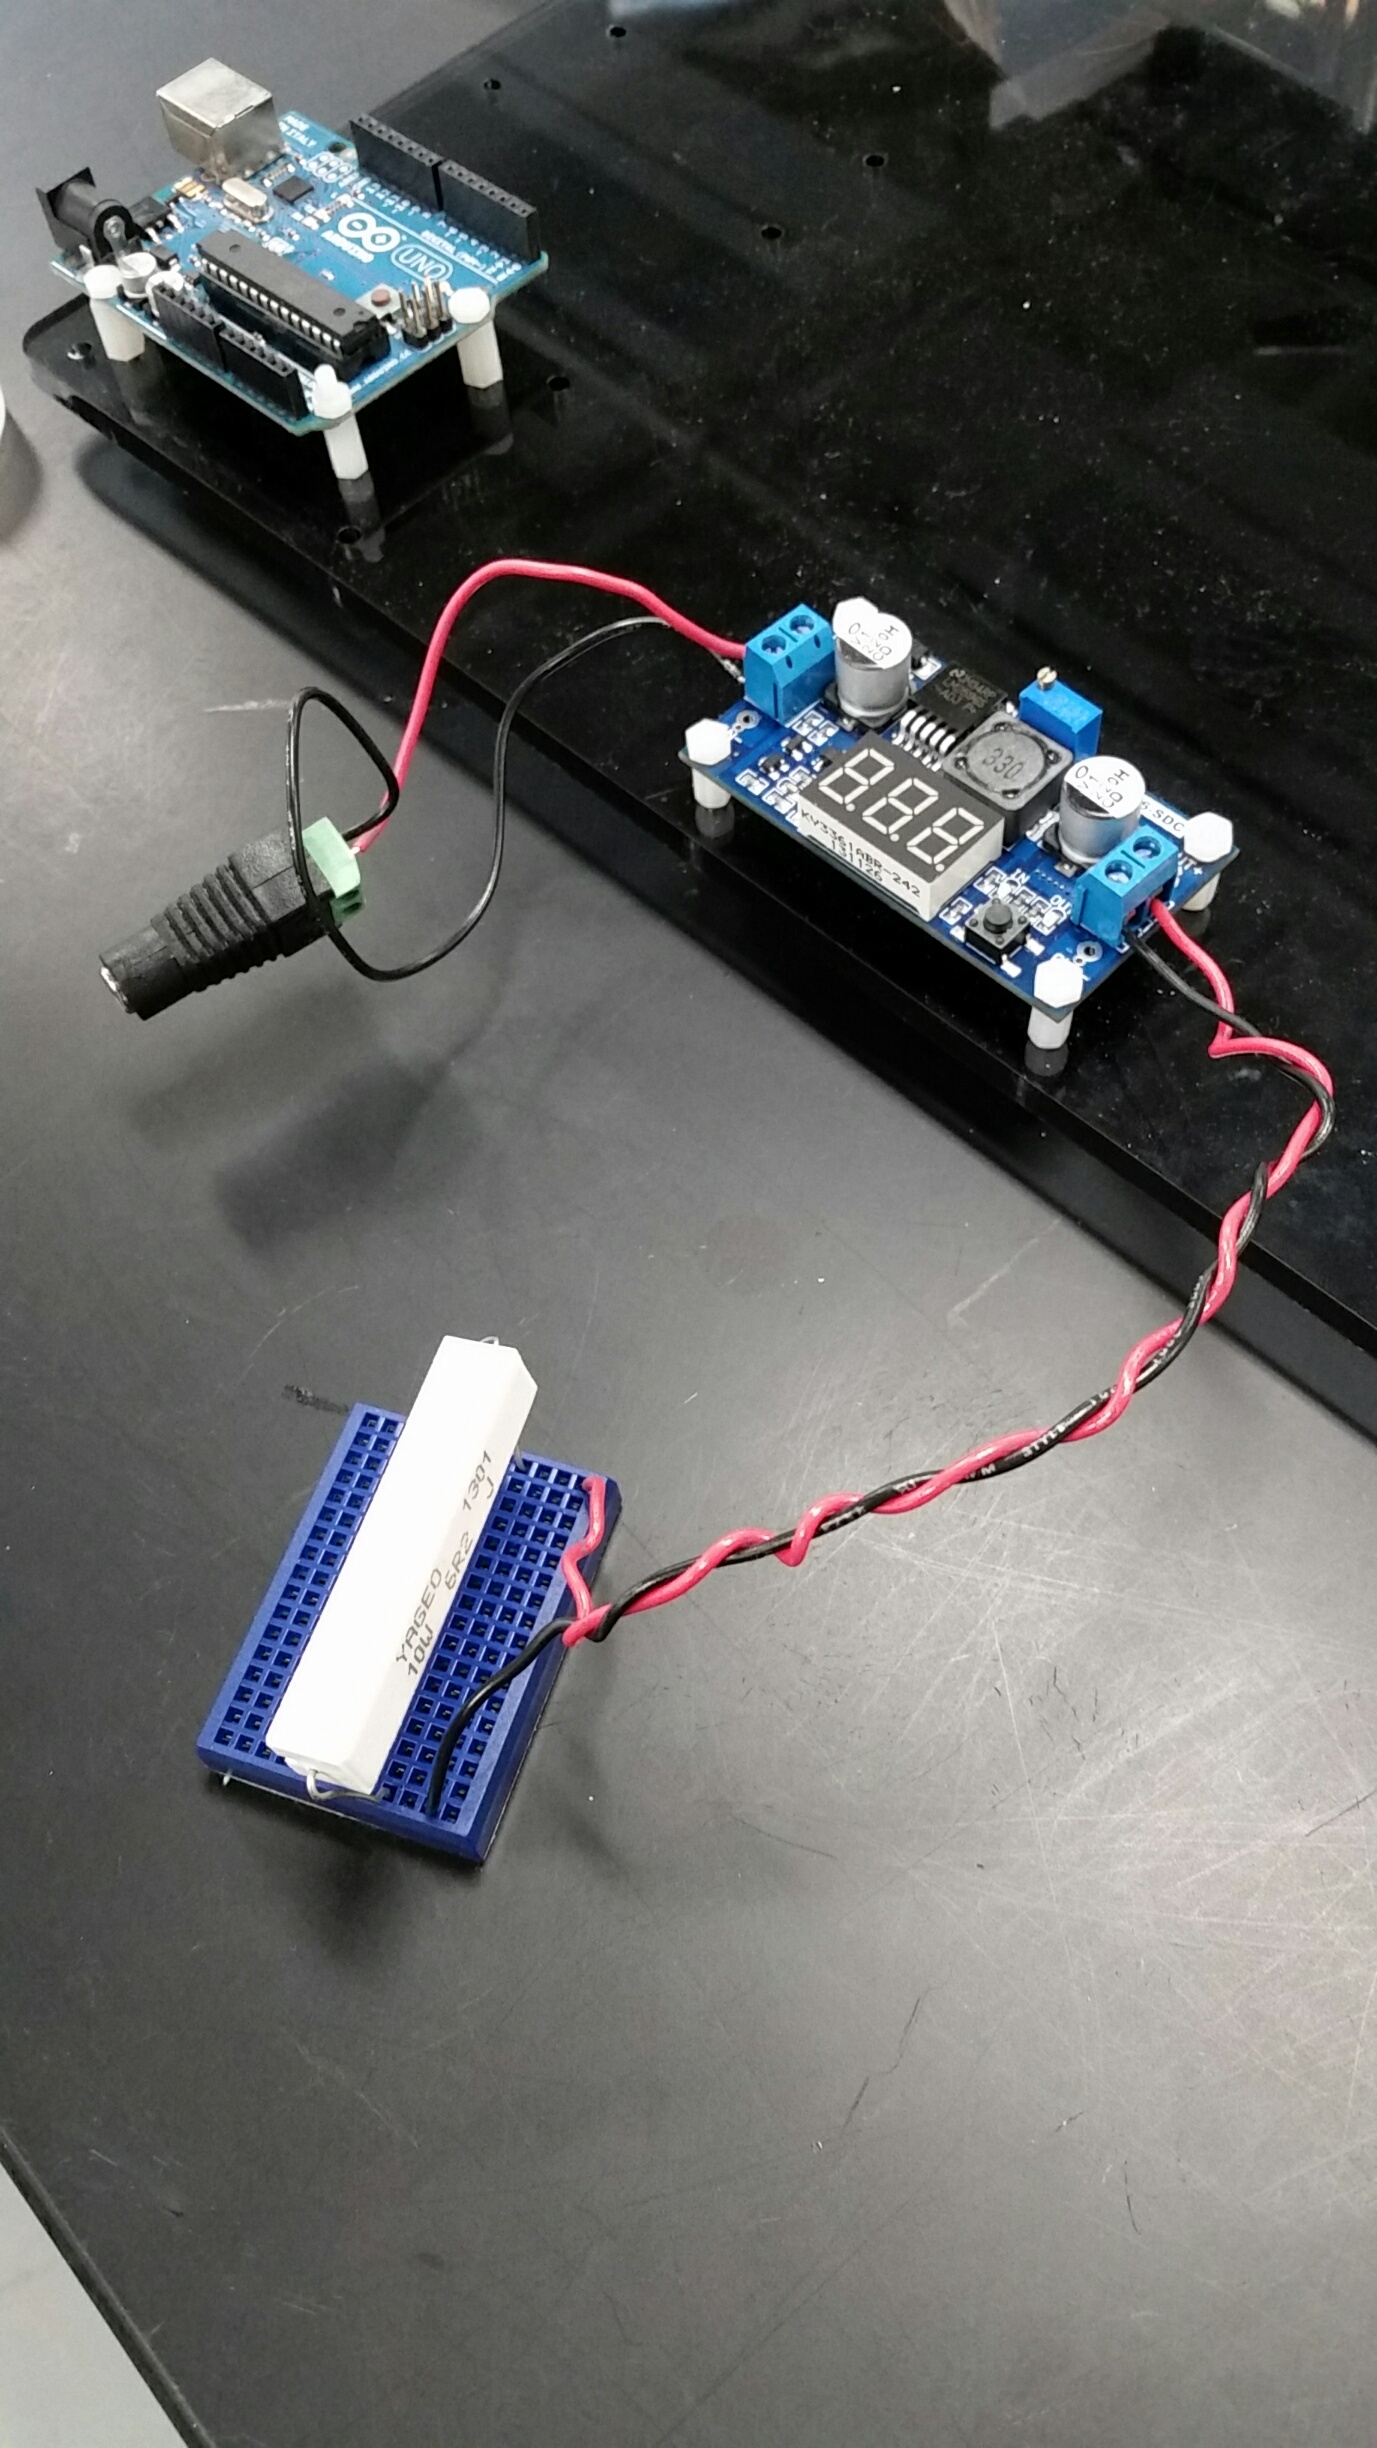
\includegraphics[width=3in ]{figures/power_resistor}
\caption{Image showing power resistor connections.}
\label{fig:power.resistor}
\end{figure}

\item Grab a $10k\Omega$ resistor and use the DMM to measure its exact resistance. $10k\Omega$ is only a nominal value: How can you tell the tolerance on it?
\item Using a breadboard, wire your thermistor according to the schematic provided in Figure~\ref{fig:thermistor.schematic}. You'll need to connect a ground, provide 5V power, and read voltages of your voltage divider.\footnote{Because the 5V power is only nominal, you need to measure the actual value so you can calculate the resistance of the thermistor accurately.} You’ll want the thermistor to be easily moved, so put it at the end of a two-wire ribbon cable.

\begin{figure}
\centering
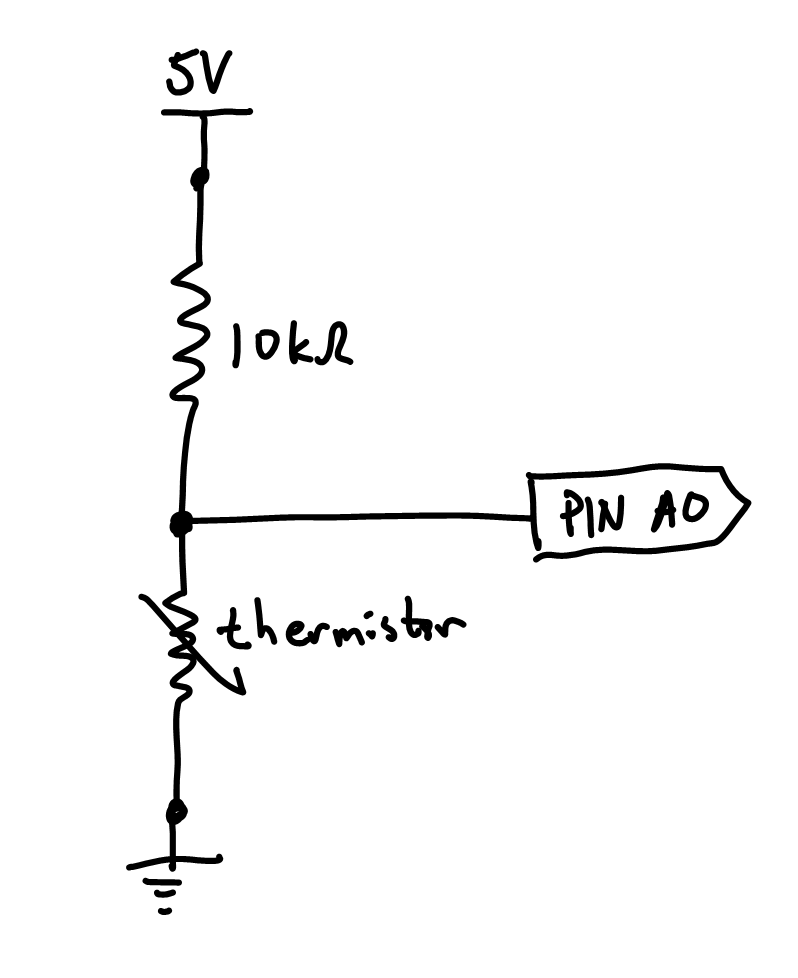
\includegraphics[width=2.5in ]{figures/thermistor_uno.png}
\caption{Schematic for temperature sensor circuit.}
\label{fig:thermistor.schematic}
\end{figure}

\item Plan how you will arrange your heater and temperature sensor in you plastic container. Note that arranging the heater and sensor is not an exact science, but you probably don't want the temperature sensor too near the heater, neither do you want it too close to a wall. Also, creating a short circuit in any of the components would be decidedly bad. {\bf The power to the temperature sensor and the heating resistor must be kept separate at all times or you risk frying the Uno!} The thermistors aren't free, either.
\item Plug in your power supply and let your power resistor heat up, \emph{but do not put it in your enclosure yet.} {\bf Be careful! It will get hot!} Not third-degree burns hot, but drop it if you grab it hot. Let the heater warm up for a good 5-10 minutes.
\item While the heater is warming, calibrate your thermistor. Though the \emph{change} in resistance is guaranteed by the manufacture, the nominal resistance is not. Therefore, you must find $R_0$ in Equation~\ref{eq:thermistor} at a known value of $T_0$. Use a DMM to measure the output voltage of your circuit and find the resistance of the thermistor. We'll assume the exterior temperature to be constant for the rest of the experiment.
\item When ready, reset the Uno by pressing the rest button and place your sensor in the enclosure. The experiment will take on the order of 20 - 30 minutes, so you may want to call over your instructor to confirm that you're properly set up before you start. The data collection process is a bit long, so if you proceed without your professor's blessing, you risk wasting time repeating the experiment.
\item Sit back and relax while the Uno does all the work for you. Now might be a good time to go buy your TA a fancy coffee product. You can also get started on the post-processing in Section~\ref{sec:post}.
\item Periodically check to see that your system has reached steady-state, since this is important for determining $K_s$. If it hasn't, let it run a bit longer. Note that if you disable the “Autoscroll” check box in the Serial Monitor, you can scroll up to see if the ADC reading is still changing.

\vspace{0.25in}
Steady-state temperature, $T_{in}$: \rule{2in}{0.4pt}
\vspace{0.25in}
\item When the system has reached steady-state, grab the data from the Serial Monitor for post-processing. You can do this by disabling the Autoscroll in the Serial Monitor and cutting and pasting the data to a file on your computer -- not particularly high-tech, but it’ll work.
\end{enumerate}

\clearpage

\section{Post processing}
\label{sec:post}
Due Monday, Feb. 5. Submit as a hard-copy, one per team. {\bf Answers without proper units will be marked incorrect.}
\begin{enumerate}
\item Import your data file into the data processing software of your choice: a spreadsheet, MATLAB, JAVA program, or similar. Convert the ADC readings to voltages and use those to find resistance of the thermistor at each timestep. Finally, convert the resistance to temperatures. If you reset the Uno when you started the experiment, then your timestamps should line up. If not, you’ll have to manually adjust them so that $t=0$ when you first put the power resistor in the container.
\item Using the calculated value of $Q_{i}$ and the steady-state value for $T_{i}$, find $K_s$.

\vspace{0.25in}
$K_s$: \rule{2in}{0.4pt}
\vspace{0.25in}

\item Calculate the time it took for the temperature differential between inside and outside to reach 63.2\% of the steady-state difference. As we’ll discuss more next week, this is one way to calculate the \emph{rise-time} of the system (why 63.2\%?). Use the rise time to find $C_{in}$ for your model.

\vspace{0.25in}
Rise-time: \rule{2in}{0.4pt}
\vspace{0.25in}

\vspace{0.25in}
$C_i$: \rule{2in}{0.4pt}
\vspace{0.25in}


\item Create another data set that corresponds to your parameterized model. That is, put $C_{i}$, $K_s$, and $Q_{i}$ into the solution of the governing equation (Equation \ref{eq:solution}) and plot the resulting curve on the same graph as your experimental data. How well does it compare to the collected data? Can you adjust the parameters to qualitatively improve the fit?% {\bf You must show your results to the instructor or lab assistant.}
%\item Gather as much information on uncertainties as you can. Carefully consider each component of your experiment and estimate the potential errors of that component. You should consult data sheets for the sensor and power resistor and use reason to assess other factors (eg, what's the precision on the voltage regulator?). Use an appropriate "worst-case scenario" to find bounds on $K$ and $C$. You may assume the error in the Analog Discovery's oscilloscope is negligible in comparison to the error in the temperature sensors.
\item Submit a graph comparing your actual data to your parameterized model. Fill in the table below with both the calculated values of the coefficients and the “best-fit’ values after adjustment.

\begin{table}[htp]
\begin{center}
\begin{tabular}{c|c|c}
Parameter & Calculated & Best-fit\\
\hline
$K_s$ & & \\
$C_{i} $ & & \\
$Q_{i} $ & & \\
\end{tabular}
\end{center}
\caption{Model parameters.}
\label{default}
\end{table}%

\item For each parameter in our model, $C_i$, $K_s$, and $Q_i$, how would raising them affect the steady-state temperature in a heating scenario, all else being equal? Fill in Table~\ref{tab:parameter.changes}.
\begin{table}[htp]
\begin{center}
\begin{tabular}{c|c}
Parameter & Effect on steady-state temperature\\
\hline
$K_s\uparrow$ & \\
$C_{i}\uparrow$ & \\
$Q_{i}\uparrow$ & \\
\end{tabular}
\end{center}
\caption{Effect of raising model parameters.}
\label{tab:parameter.changes}
\end{table}%

\item The greenhouse from IKEA are substantially larger than the ones we used for the in-lab experiment. It is not always easy to apply a small-scale experiment to a larger one, but it is often possible to approximate $K$ by scaling according to surface area (assuming the thermal conductance of the material per unit area doesn't change, which is reasonable in this case). Estimate the surface area of the IKEA greenhouse and estimate $K_s$ for the full-scale model. How big of a heater would be needed to maintain a 10C temperature differential above the outside temperature?
\vspace{2in}
\item Find the resistance tolerance, $\Delta R/R$, on the \href{http://en.tdk.eu/inf/50/db/ntc_13/NTC_Leaded_disks_K164.pdf}{\underline{datasheet for the thermistor}}. (we’re using the ‘J’ model). Calculate the error bounds for the steady-state temperature, in Celsius. Calculate the resultant error bounds on $K$. Ignore all other sources of error.
%\item Using the worst-case scenario for February in Charlottesville (-18C outdoor temperature) calculate the heating power needed to maintain an inside temperature of 5C at steady-state for the full-scale model. Will our 50W power supplies be big enough? If so, what would be the inside temperature under the worst-case scenario? If not, what could you do to prevent the inside from getting too cold? Give three suggestions.
%\vspace{1in}
\end{enumerate}

\clearpage
\section{Pre-lab Worksheet (5 points)}
\label{sec:prelab}
To be turned in before the start of the lab. This is an individual assignment.
\begin{enumerate}
\item Which do you think would have a higher value of $K$: an old, leaky house or a new, well-sealed house of the same size?
\vspace{0.75in}
\item Which do you think would have a higher value of $K$: a small house or a large house with similar construction?
\vspace{0.75in}
\item Calculate the current flowing through a 10$\Omega$ resistive element if the voltage applied across the terminals is 5V. Calculate the power that is dissipated under the same conditions.
\vspace{0.75in}
\item A 5$\Omega$ resistive element is rated for 100W. What is the largest voltage differential that can be applied to it without exceeding the power rating? How many amps will flow through it at that voltage?
\vspace{0.75in}
%\item You're given some wire with a resistance of 4$\Omega/m$ and you want to use it to generate 48W through resistive heating. The wire can only tolerate 2A and you can supply 12V to it. Devise an arrangement that produces the necessary power without exceeding the current limitations.
%\vspace{1in}
\item During the dreaded ``Polar Vortex'', the heater in my house could not bring the indoor temperature to the desired set-point. After running long enough to reach steady-state, the inside only got up to 19C. Assuming a constant outside temperature of -18C (it was pretty cold for a long time), determine $K$ for my house if my heater puts out 15,000W.
\vspace{0.75in}
\item 10kg of water at 50C is placed in an insulated box with an overall heat transfer coefficient of 1W/C. The box is in a room at 20C. How long will it take for the temperature of the water to drop to 30C? Ignore the mass of the insulation -- use only the mass of water to find $C$ for the system.
\vspace{0.75in}
%\item In Carryer \emph{et al.}, do Problem 13.6. Attach your plot at the end.%Consult the datasheet for the B57164K103J thermistor that you will use in this lab...
%\vspace{1in}
\item Substitute Eq.~\ref{eq:solution} into Eq.~\ref{eq:gov.eq} to show that it is a solution to the governing equation when $T_{o}$ and $Q_{i}$ are constant. Do not solve Eq.~\ref{eq:gov.eq} ``from scratch.'' Just prove that Eq.~\ref{eq:solution} is a solution.
\vspace{1.5in}
\item Derive the steady-state solution for Eq.~\ref{eq:solution}, as determined by taking the limit of Eq.~\ref{eq:solution} as $t\rightarrow\infty$. Assume $T_{o}$ and $Q_{i}$ are constant.
\vspace{1.5in}
\item Derive the steady-state solution from Eq.~\ref{eq:gov.eq}, as determined by setting the derivative to zero and solving the remaining algebraic expression. Assume $T_{o}$ and $Q_{i}$ are constant.
\vspace{1.5in}
\item Given the voltage divider in Figure~\ref{fig:voltage.divider.prelab}, calculate the voltage, $V_B$, for the nominal resistor values. Calculate the range of possible values using the specified tolerances of the resistors.
\vspace{1.5in}
\item How much current can the voltage regulator on a SparkFun RedBoard reliably supply?
\vspace{1.5in}
%\item Theoretical model.
%\vspace{1.5in}
\begin{figure}[htbp]
\begin{center}
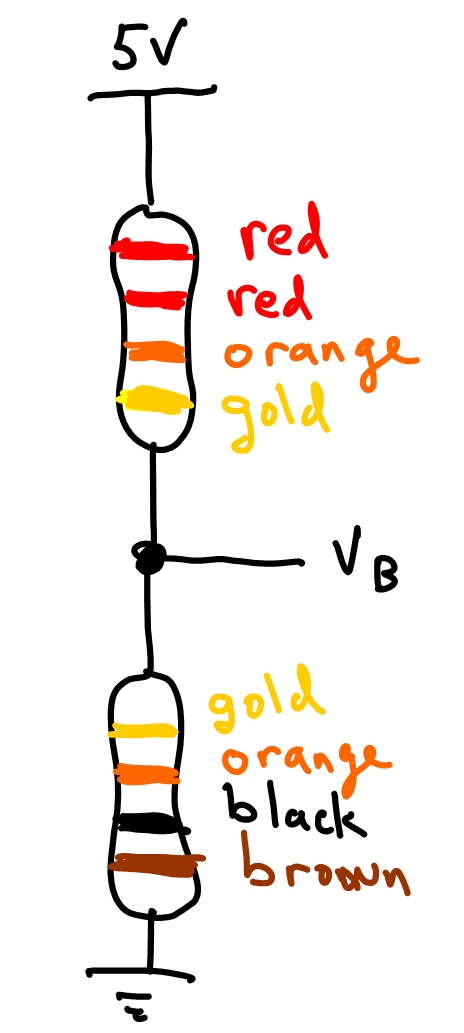
\includegraphics{figures/prelab_divider}
\caption{Voltage divider for the pre-lab.}
\label{fig:voltage.divider.prelab}
\end{center}
\end{figure}

\end{enumerate}



\end{document}

